% covtl-pipeline --- Multi-Speaker Registry Manual
% SPDX-License-Identifier: GPL-3.0-or-later
% Copyright (C) 2026 Frédéric Berthommier
%
% Compile with plain pdflatex (standard packages only):
%     pdflatex speakers.tex && pdflatex speakers.tex
% (run twice for the table of contents and cross references)

\documentclass[11pt,a4paper]{article}

% --- Packages (same visual language as docs/manual.tex) ---
\usepackage[T1]{fontenc}
\usepackage[utf8]{inputenc}
\usepackage{lmodern}
\usepackage{graphicx}
\usepackage{xcolor}
\usepackage{geometry}
\usepackage{amsmath}
\usepackage{amssymb}
\usepackage{tcolorbox}
\tcbuselibrary{listings, breakable, skins}
\usepackage{booktabs}
\usepackage{tabularx}
\usepackage{enumitem}
\usepackage{array}
\usepackage{longtable}
\usepackage{fancyhdr}
\usepackage{titlesec}
\usepackage{listings}
\usepackage{needspace}
\usepackage[
    colorlinks=true,
    linkcolor=blue!60!black,
    citecolor=blue!50!black,
    urlcolor=blue!70!black,
    bookmarks=true,
    bookmarksnumbered=true,
    unicode=true,
    pdftitle={covtl-pipeline Multi-Speaker Registry},
    pdfauthor={Frederic Berthommier},
    pdfsubject={Five VocalTractLab speakers: provenance, adaptation and switching in covtl-pipeline},
    pdfkeywords={VocalTractLab, speaker adaptation, MRI, area function, multi-speaker registry, articulatory synthesis, COVTL}
]{hyperref}

\geometry{a4paper, top=2.5cm, bottom=2.5cm, left=2.5cm, right=2.5cm}
\setlength{\headheight}{14pt}

\pagestyle{fancy}
\fancyhf{}
\fancyhead[L]{\small\itshape covtl-pipeline --- Multi-Speaker Registry}
\fancyhead[R]{\small v1.1.0}
\fancyfoot[C]{\thepage}
\renewcommand{\headrulewidth}{0.3pt}
\renewcommand{\footrulewidth}{0pt}

\titleformat{\section}{\needspace{0.25\textheight}\Large\bfseries\color{blue!50!black}}{\thesection}{0.6em}{}
\titleformat{\subsection}{\needspace{6\baselineskip}\large\bfseries\color{blue!40!black}}{\thesubsection}{0.5em}{}
\titleformat{\subsubsection}{\needspace{5\baselineskip}\normalsize\bfseries}{\thesubsubsection}{0.4em}{}

% --- Listings ---
\definecolor{codebg}{HTML}{F5F5F5}
\definecolor{codeframe}{HTML}{CCCCCC}
\definecolor{codecomment}{HTML}{6A737D}
\definecolor{codekeyword}{HTML}{D73A49}
\definecolor{codestring}{HTML}{032F62}
\lstdefinestyle{shell}{
    backgroundcolor=\color{codebg},
    frame=single,
    rulecolor=\color{codeframe},
    basicstyle=\ttfamily\footnotesize,
    commentstyle=\color{codecomment}\itshape,
    keywordstyle=\color{codekeyword}\bfseries,
    stringstyle=\color{codestring},
    showstringspaces=false,
    breaklines=true,
    breakatwhitespace=true,
    numbers=none,
    xleftmargin=4pt,
    xrightmargin=4pt,
    framexleftmargin=4pt,
    framexrightmargin=4pt,
    language=bash,
    morekeywords={python, pip, pytest, git, curl}
}
\lstdefinestyle{verbatim}{
    backgroundcolor=\color{codebg},
    frame=single,
    rulecolor=\color{codeframe},
    basicstyle=\ttfamily\footnotesize,
    showstringspaces=false,
    breaklines=true,
    breakatwhitespace=true,
    numbers=none,
    xleftmargin=4pt,
    xrightmargin=4pt,
    framexleftmargin=4pt,
    framexrightmargin=4pt
}

% --- tcolorbox callouts ---
\newtcolorbox{callout}[1][]{
    colback=blue!5,
    colframe=blue!50!black,
    fonttitle=\bfseries,
    title={#1},
    breakable=true
}
\newtcolorbox{warning}[1][]{
    colback=orange!10,
    colframe=orange!70!black,
    fonttitle=\bfseries,
    title={#1},
    breakable=true
}

\newcommand{\speakerfile}[1]{\texttt{#1.speaker}}
\newcommand{\code}[1]{\texttt{#1}}

\widowpenalty=10000
\clubpenalty=10000
\emergencystretch=1.5em
\tolerance=2000
\newcommand{\sectionbreak}{\needspace{0.3\textheight}}

\title{\vspace{-1cm}\Huge\bfseries\color{blue!50!black} The Multi-Speaker
Registry\\[0.3em]
\Large\mdseries\color{black!70} Five VocalTractLab speakers: provenance,
adaptation and switching}
\author{\large Frédéric Berthommier\\[0.3em]
\small\texttt{fberthommier@users.noreply.github.com}}
\date{\small Version 1.1.0 --- September 2026\\[0.2em]
\textit{Licensed under GPL-3.0-or-later}}

\begin{document}
\maketitle
\thispagestyle{empty}

\begin{abstract}
\noindent
covtl-pipeline ships \textbf{five VocalTractLab speakers} and makes
switching between them a single reversible command:
\code{python install\_speaker.py install <name>}. This manual, one of
the five manuals of the repository, documents the \emph{speaker
registry} (the on-disk source of truth and the four software layers a
switch must keep coherent) and the provenance of each speaker: the
reference speaker \speakerfile{JD3}; \code{s1} and \code{s2}, built
from the public-domain Dresden Vocal Tract Dataset (DVTD) MRI meshes
by area-function measurement, anatomy mapping and a two-phase
adaptation to the Berthommier COVTL model; and \code{m01} and
\code{w02}, the official VTL~2.4 speakers made loadable by the
value-preserving ``Option~A'' schema patch. Every step is stated with
the numbers obtained on the real data, and the numbered defect
catalogue (D1--D21) records what the transfers taught us.
\end{abstract}

\vspace{0.5em}
\tableofcontents
\vspace{1em}

%==============================================================================
\section{Introduction}\label{sec:intro}
%==============================================================================

\subsection{What a VTL speaker file is}

\textbf{VocalTractLab} (VTL, Peter Birkholz, TU Dresden) is an
articulatory speech synthesizer: the vocal tract is reduced to 40
tube sections, driven by 19 tract parameters and an 11-parameter
geometric glottis, and audio is rendered at 44.1\,kHz. A VTL
\emph{speaker} is a single XML file (conventionally \speakerfile{NAME})
that fixes everything speaker-specific:

\begin{itemize}[leftmargin=1.5em]
\item the \textbf{anatomy}: rest positions, ranges (\texttt{min},
      \texttt{max}) and neutral values of the 19 tract parameters
      (hyoid, jaw, lips, tongue body/tip and lateral shapes, velum,
      teeth geometry), plus the palate contour and lip geometry;
\item the \textbf{glottis models}: static parameters and the 11
      control parameters (each with range, neutral value and
      metadata), plus a repertoire of named \emph{shapes}
      (\texttt{modal}, \texttt{breathy}, \texttt{creak}, \ldots);
\item a repertoire of named \textbf{tract shapes} (\texttt{a},
      \texttt{i}, \texttt{s}, \ldots) --- vectors of the 19 tract
      parameters used as starting gestures.
\end{itemize}

covtl-pipeline does not read these numbers directly: it synthesizes
with the \textbf{Berthommier COVTL model}, whose speaker-dependent
quantities (the 15 polar-plane projection coefficients
\(c_0, c_1, c_2\) per parameter, phoneme targets, glottal presets,
\texttt{f0\_default}, effort bounds) live in a generated Python
module, \code{constants.py}. Producing that module from a
\speakerfile{} file is called \emph{adaptation}
(\S\ref{sec:adapt}).

\subsection{The five speakers}

\begin{table}[ht]
\centering
\small
\begin{tabular}{@{}lllrlr@{}}
\toprule
\textbf{name} & \textbf{origin} & \textbf{sex} & \textbf{source data} &
\textbf{VTL (cm)} & \textbf{f0 default (Hz)} \\
\midrule
\code{jd3} & VTL 2.4 reference & male & official \texttt{VTL2.4.zip} & 17.00 & 102.216 \\
\code{s1}  & DVTD subject 1 & male & MRI, 39 y, 1.85 m & 20.04 & 114.908 \\
\code{s2}  & DVTD subject 2 & female & MRI, 32 y, 1.64 m & 15.08 & 181.008 \\
\code{m01} & official VTL 2.4 & male & official \texttt{VTL2.4.zip} & --- & 120.000 \\
\code{w02} & official VTL 2.4 & female & official \texttt{VTL2.4.zip} & --- & 232.458 \\
\bottomrule
\end{tabular}
\caption{The five speakers of the registry. VTL is the mean vocal-tract
length over tense vowels (measured on the source data where
available); m01/w02 anatomies are kept exactly as distributed (not
re-measured).}
\label{tab:speakers}
\end{table}

JD3 is the speaker on which the pipeline was calibrated; it serves as
the template for both the DVTD construction (\S\ref{sec:dvtd}) and
the adaptation chain (\S\ref{sec:adapt}), and it is the only speaker
that follows the language pack (its vowel targets are re-calibrated
per language; \code{docs/language\_pack.pdf}). The four other
speakers are shipped with their \textbf{native} vowel targets and are
validated in that regime.

\begin{figure}[ht]
\centering
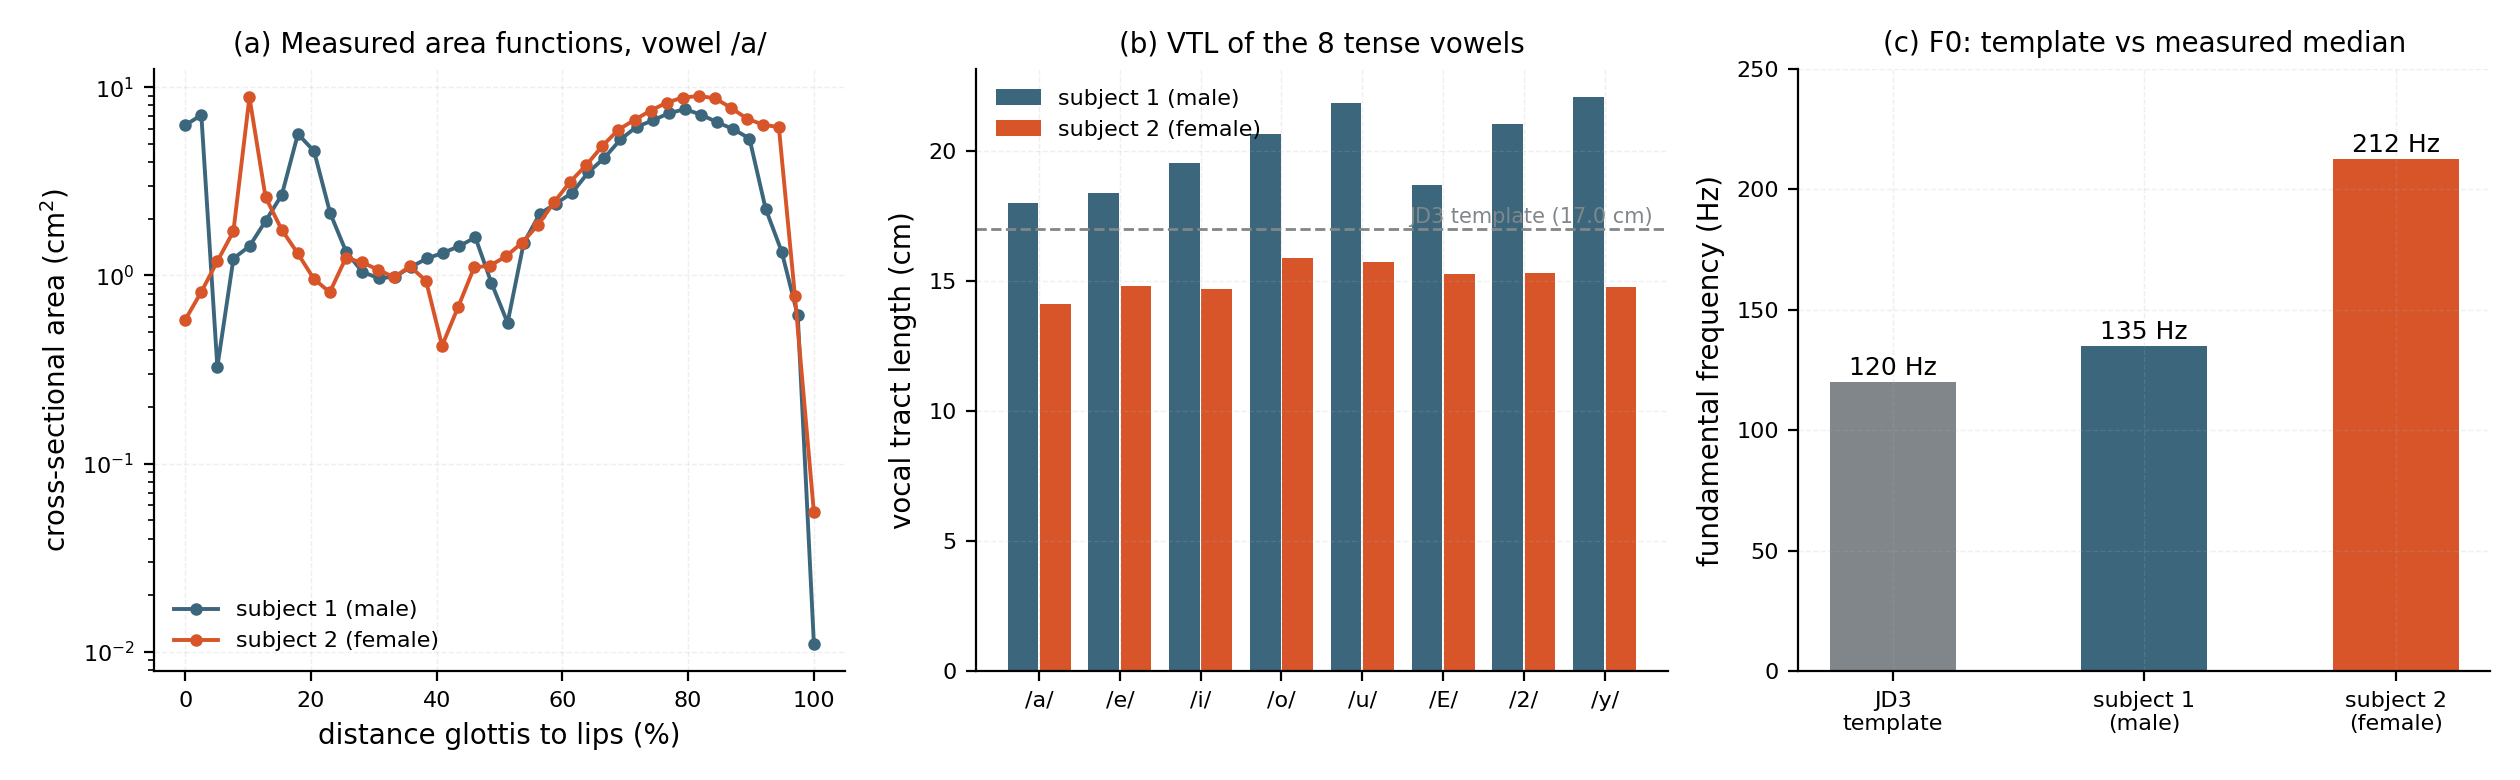
\includegraphics[width=\textwidth]{figures/figure_doc_overview.png}
\caption{Source-data overview for the DVTD subjects. (a) Measured
area functions of sustained /a/ (s1 male, s2 female), glottis to lips.
(b) Vocal-tract lengths of the eight tense vowels against the JD3
template (dashed line). (c) F0 templates and measured medians (JD3
120\,Hz; s1 135\,Hz; s2 212\,Hz).}
\label{fig:overview}
\end{figure}

%==============================================================================
\section{The registry: switching speakers in one command}\label{sec:registry}
%==============================================================================

\subsection{The registry as a single source of truth}

The directory \code{vtl\_synth/data/speakers/} holds everything:

\begin{center}
\small
\begin{tabularx}{\textwidth}{@{}lX@{}}
\toprule
\textbf{file} & \textbf{role} \\
\midrule
\code{registry.json} & one entry per speaker: file names,
\texttt{f0\_default}, description, SHA-256 of both files \\
\code{ACTIVE\_SPEAKER} & one-line marker naming the active speaker \\
\code{jd3.speaker}, \code{s1.speaker}, \ldots & the speaker files \\
\code{jd3\_constants.py}, \code{s1\_constants.py}, \ldots &
the constants sources \\
\bottomrule
\end{tabularx}
\end{center}

The design rule: the installed \code{core/constants.py} is always a
\emph{bit-exact copy} of a registry source (its SHA-256 identifies
the speaker), while the active \emph{name} is read from the separate
marker. \code{ACTIVE\_SPEAKER} is not part of the package: create it
once with \code{python install\_speaker.py list}.

\subsection{Four layers, one command}

A speaker switch must coordinate four layers:

\begin{enumerate}[leftmargin=1.8em]
\item \textbf{geometry / glottis / f0 default}: the installed
      \code{core/constants.py} (swapped file);
\item \textbf{orthogonal branch} (VS, VO, TS3, tongue-root context
      maps): the \speakerfile{} file resolved through the registry and
      read at each call;
\item \textbf{audio + SVG/video}: the \code{vocaltractlab-cython}
      wheel loads its own packaged speaker resource at import time;
      the installer swaps that resource --- the effect applies to the
      \emph{next} process;
\item \textbf{regression baselines}: one file per speaker
      (\code{regression\_baselines\_<spk>.json}), checked
      by the parameterized test suite and regenerated with
      \code{scripts/regen\_baselines.py}.
\end{enumerate}

\begin{lstlisting}[style=shell]
python install_speaker.py list            # speakers + active one
python install_speaker.py install s2      # swap constants + wheel resource
python install_speaker.py restore         # back to jd3 (bit-exact)
python install_speaker.py status          # hashes, layer coherence
\end{lstlisting}

Each \code{install} runs seven steps: registry lookup, hash check of
the source constants, backup manifest (SHA-256), constants copy with
post-copy hash verification, \code{ACTIVE\_SPEAKER} marker write,
wheel-resource swap with hash verification, and a smoke test in a
\emph{fresh subprocess} (synthesis of \code{a i u} plus a check of
the speaker announcement). Any error triggers automatic rollback ---
the tree is never left half-installed.

\subsection{The announcement and the f0 default}

Every synthesis announces which speaker each layer uses, e.g.

\begin{lstlisting}[style=verbatim]
Speaker actif : s2 (DVTD sujet 2 female)  constants=23dd28dd4cf4
                f0_default=181.008 Hz
                geometry: s2  ortho: s2  audio wheel: s2  video: s2
\end{lstlisting}

and appends explicit warnings when layers disagree (a process started
before a wheel swap, or an incomplete install). The CLI resolves the
default F0 from the \emph{active} speaker constants
(102.216\,Hz for jd3, 114.908 for s1, 181.008 for s2, 120.0 for m01,
232.458 for w02); a forced \texttt{-f0} value is announced. Proof on
s2: \texttt{-f0 181.008} measures a median F0 of 183.5\,Hz in the
output signal.

\begin{callout}[Baselines are speaker-relative]
The end-to-end baselines encode the synthesis output of
\emph{one speaker}. \code{restore --check-baselines} verifies the
jd3 reference bit-exactly after a restore; after any voluntary
modification of the signal path (speaker work, language-section
changes), regenerate the reference with
\code{scripts/regen\_baselines.py}. Per-speaker files keep every
speaker checkable independently.
\end{callout}

\subsection{Interaction with the language pack}

The language pack (\code{setup\_lang.py}) edits the managed LANG
SECTION (vowel targets, effort gains) \emph{inside} the installed
\code{constants.py}. Its calibration is anchored to JD3: the
language-management commands carry a guard that (re)installs jd3
before touching the section, and a speaker swap carries an existing
LANG SECTION over to the target constants. The four non-reference
speakers are shipped and validated with native targets --- keep the
default language \code{en} to work in the native regime. The exact
workflows are described in \code{docs/language\_pack.pdf}
(\S\,\emph{Integration and the JD3 guard}) and
\code{docs/expressive\_prosody.pdf} (\S\,\emph{Interaction with the
speaker setup}).

%==============================================================================
\section{Provenance I --- building s1/s2 from public MRI (DVTD)}\label{sec:dvtd}
%==============================================================================

\subsection{The data source}

The \textbf{Dresden Vocal Tract Dataset} (DVTD) is a public
collection of sustained-phonation MRI of two subjects, published as
full-resolution surface meshes.

\begin{center}
\small
\begin{tabular}{@{}ll@{}}
\toprule
\textbf{item} & \textbf{value} \\
\midrule
Authors & P.~Birkholz, S.~K\"urbis, S.~Stone, P.~H\"asner,
R.~Blandin, M.~Fleischer \\
Reference & Birkholz et al.\ 2020, \emph{Sci.\ Data} 7:255,
\code{doi:10.1038/s41597-020-00597-w} \\
Archive & \code{dvtd.zip}, 1\,129\,467\,424 bytes (1.13 GB) \\
DOI & \code{10.6084/m9.figshare.11897187.v1} \\
License & \textbf{CC0 1.0} (public domain) \\
\bottomrule
\end{tabular}
\end{center}

Per subject and per sound (22 sustained sounds: German tense/lax
vowels, fricatives, laterals, schwa), the archive provides the inner
airway surface mesh from glottis to lips, vocal-tract transfer
functions (\code{measured} and finite-element), a reference recording
of the same phonation, and manually picked anatomical landmarks
(essential for subject~1). Because the license is CC0, the derived
speakers and all measurements can be redistributed without
restriction.

\subsection{Measuring the area function on a mesh}

The measurement module works directly on the triangulated
inner-surface meshes, without re-meshing:

\begin{enumerate}[leftmargin=1.8em]
\item \textbf{Medio-sagittal plane}: found as the plane of maximal
      cut area (scan over the lateral coordinate, then refinement).
\item \textbf{2D cavity mask}: on that plane, the cavity is recovered
      by a parity test on the mesh--plane intersection segments
      (0.5\,mm step).
\item \textbf{Centerline}: tracked from the glottis end by
      contiguity through the laryngeal vestibule and pharynx (across
      velar pinches of width $\le 8$\,mm), then horizontally in the
      mouth region; smoothed and resampled at 40 stations.
\item \textbf{Areas}: each station's cross-section is the
      intersection of the mesh with the plane perpendicular to the
      centerline; all loops are summed, so the piriform fossae are
      included.
\item \textbf{Vocal-tract length (VTL)}: curvilinear length
      glottis $\to$ lips of the centerline.
\end{enumerate}

The runner measures the 22 sounds and writes, per sound, the VTL,
40 areas, palate contour, transfer-function resonances and the median
F0 of the reference recording (autocorrelation).

\begin{figure}[ht]
\centering
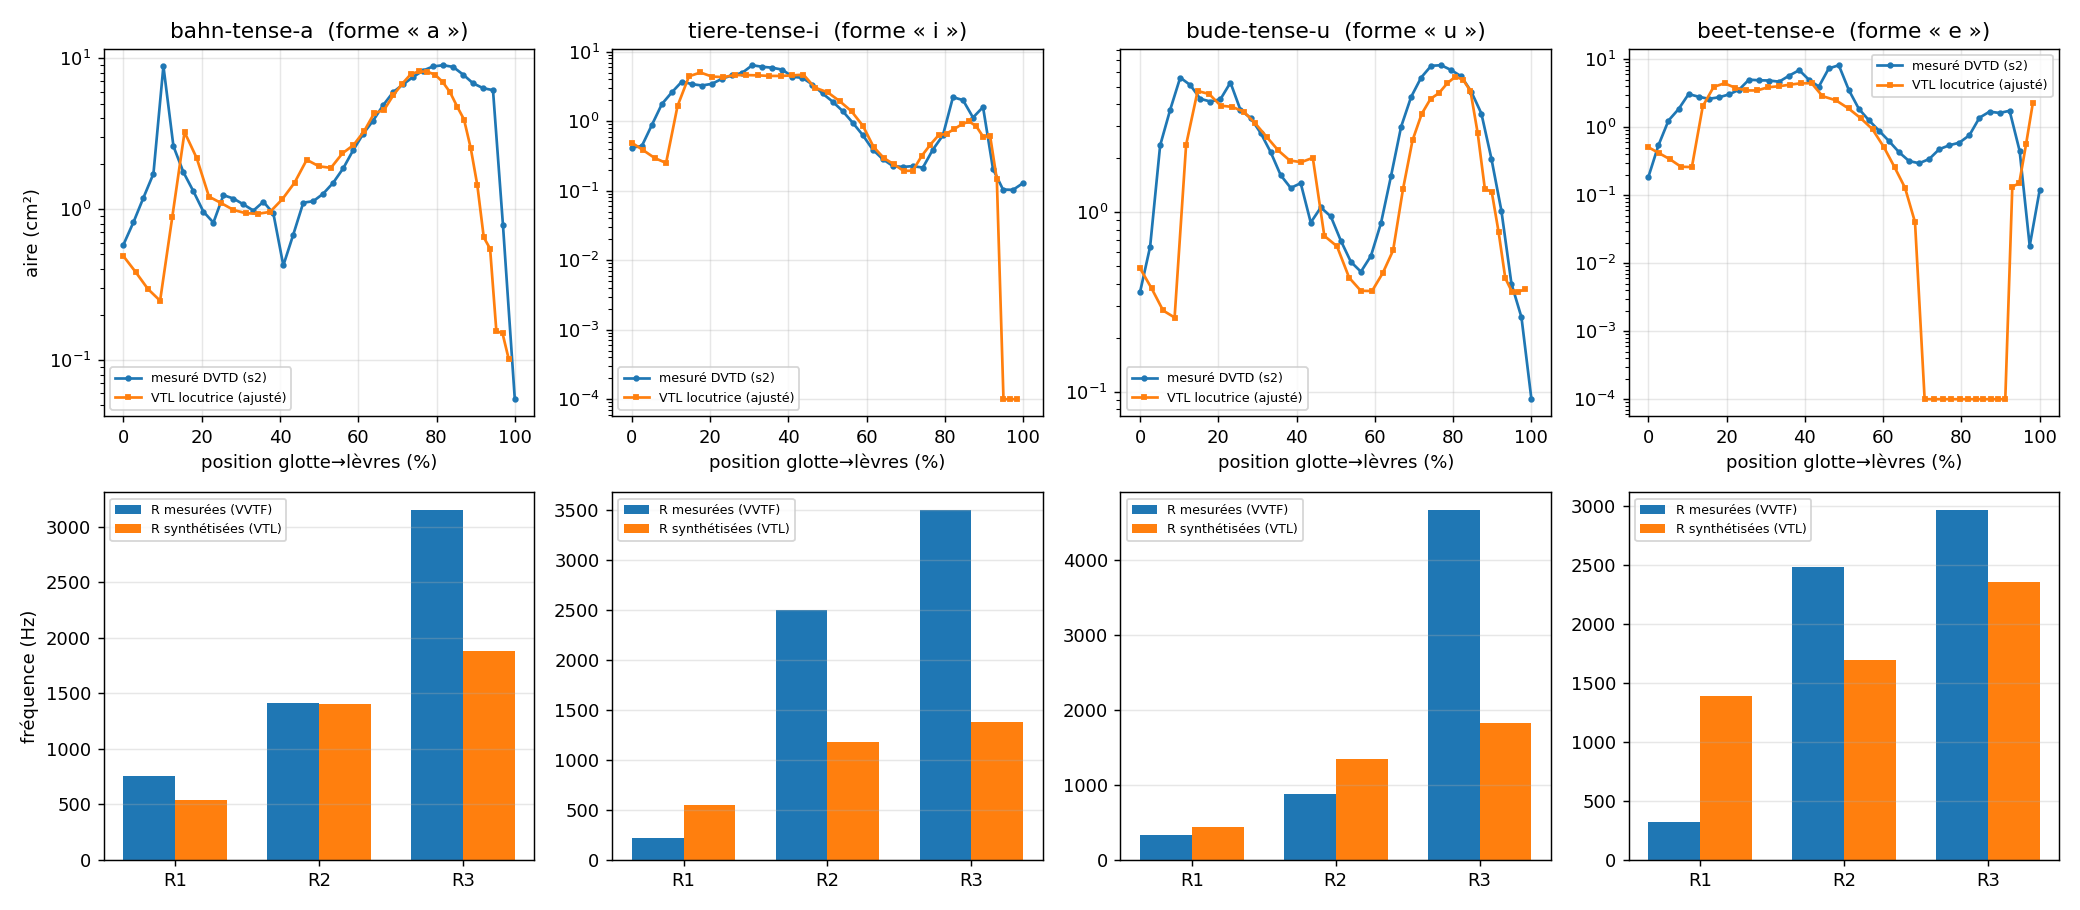
\includegraphics[width=0.94\textwidth]{figures/figure_validation.png}\\[0.4em]
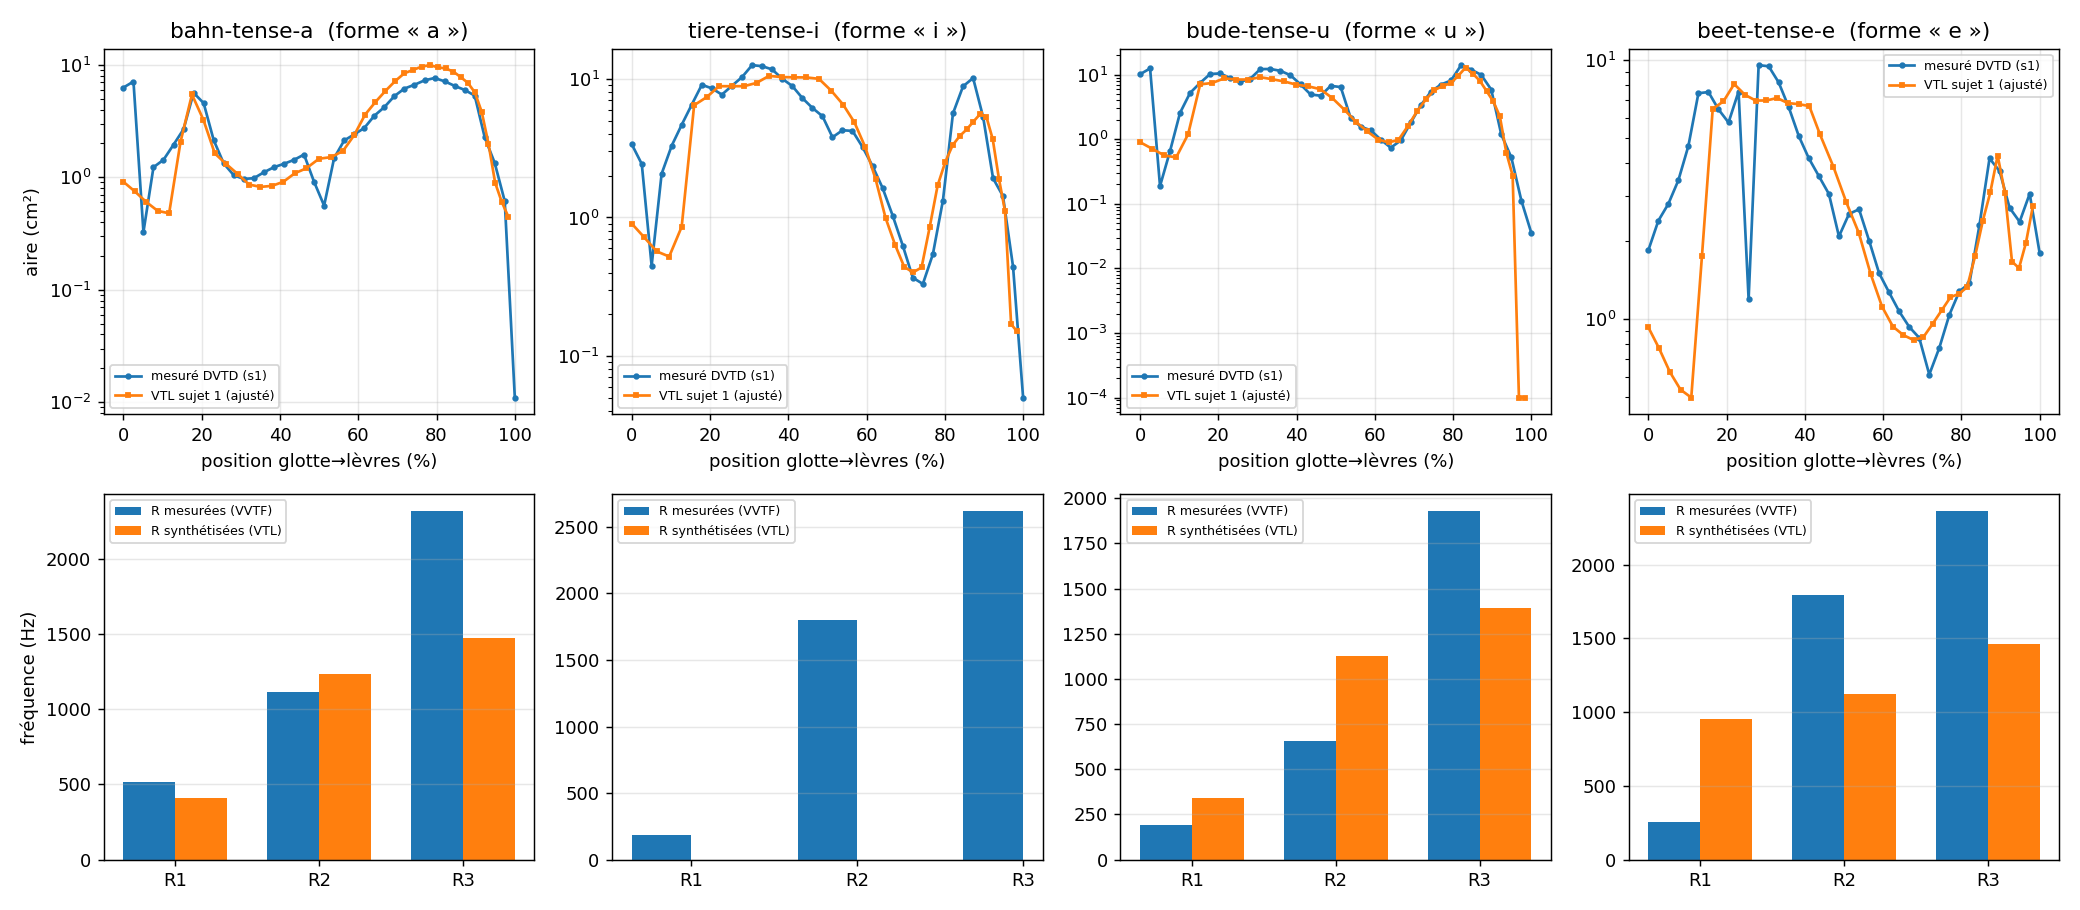
\includegraphics[width=0.94\textwidth]{figures/figure_validation_s1.png}
\caption{Validation figures for s2 (top) and s1 (bottom): measured vs
fitted area functions and measured vs synthesized resonances.}
\label{fig:validation}
\end{figure}

\subsection{Scales and anatomy mapping}

Two scalar factors drive the mapping onto the JD3 template:
\begin{equation}
s_L \;=\; \frac{\mathrm{VTL}_{\text{subject, tense vowels}}}
               {\mathrm{VTL}_{\text{JD3, same shapes}}}
\qquad
k_{f0} \;=\; \frac{f0_{\text{subject, median}}}{120~\text{Hz}} .
\end{equation}

\begin{center}
\small
\begin{tabular}{@{}lrr@{}}
\toprule
 & \textbf{s2 (female, 32 y)} & \textbf{s1 (male, 39 y)} \\
\midrule
VTL, tense vowels (range) & 15.08 cm (14.14--15.89) & 20.04 cm (18.03--22.07) \\
$s_L$                     & 0.8873 & 1.1792 \\
F0 median of recordings   & 212.5 Hz (192--231) & 134.9 Hz (115--138) \\
$k_{f0}$                  & 1.771 & 1.1242 \\
Neutral VTL of the built speaker & 15.75 cm & 18.29 cm \\
\bottomrule
\end{tabular}
\end{center}

The generator then edits the JD3 template block by block: each block
is either \emph{scaled} by $s_L$ (longitudinal anatomy, tongue rest
positions, larynx height) or \emph{kept} at the JD3 value (teeth and
lips, following the official female-speaker precedent where one
exists; jaw rest displacements), with the justification recorded per
field in a JSON journal. Subject~1 required one extra check: his 22
meshes do not share a common coordinate frame (three groups of
offsets/inclinations); the ``lips at $y$ max, glottis at $z$ min''
convention was verified sound by sound against the manually picked
lip points, and the measured 20\,cm tract was confirmed plausible by
an independent 1D transmission-line model (the s1/s2 resonance ratios
match the geometric length ratio).

\subsection{Fitting the shape repertoire and validating}

The built speaker keeps the JD3 shape repertoire as gesture skeleton
and refits the free parameters of each target shape so that the
\emph{rendered} area function matches the \emph{measured} one
(19 tract parameters per shape against the 40-station area function;
RMS of log-area 0.57--1.0). Validation compares, per sound, the
resonances of the synthesized speaker with the measured
transfer-function peaks: mean relative errors for s2 are R1 86\%,
R2 32\%, R3 41\% --- the first resonance of front vowels is the
weakest point, a known limitation of a JD3 skeleton carrying a
foreign tongue-shape repertoire. Transferability was checked by
replaying JD3 gestures unchanged: formants stay within a few percent
for back vowels and diverge on /y/ (F1 $+91\%$), quantifying how far
JD3 gestures can be reused.

The chain output is the raw mapped speaker
(\code{speaker\_\{male,female\}\_DVTD.speaker}) and, after format
normalization, the registry entries \code{s1.speaker} and
\code{s2.speaker}.

%==============================================================================
\section{Provenance II --- adapting a speaker to the COVTL model}\label{sec:adapt}
%==============================================================================

A \speakerfile{} file is not yet usable by the pipeline: adaptation
is the deterministic derivation of the \code{constants.py} module,
followed by a geometric calibration.

\subsection{Phase 1 --- articulatory adaptation}

Five stages extract everything derivable exactly from the speaker
file:

\begin{description}[leftmargin=2em]
\item[Stage 1 --- the COVTL plane (deterministic).] For each of the
  15 selectable parameters, the exact $3\times3$ linear system on the
  native /a/, /i/, /u/ shape values at the Maeda anchors
  ($\theta_a = \pi$, $\theta_i = 5\pi/3$, $\theta_u = \pi/3$) is
  solved for $P(\theta) = c_1 + A\cos\theta + B\sin\theta$, with
  $c_0 = \sqrt{A^2+B^2}$, $c_2 = \operatorname{atan2}(B,A)$.
  Validated on JD3 against the reference constants to
  $5\cdot10^{-7}$.
\item[Stage 2 --- closure and contact offsets.] Rules transferred
  from the reference calibration (all verified on JD3 to
  $<1.3\cdot10^{-4}$): lip-closure LD rule; tongue-tip ceiling TTY
  (with the $+0.15$ apical-occlusion bonus of /d, t/); tongue-body
  raising TCY ($+0.25$ for the velar occlusion of /g, k/); glottal
  flutter and aspiration zeroed (except the \code{hoarse2} preset).
\item[Stage 3 --- vowels.] /a/ is the anchor $(1, \pi)$; /i/ and /u/
  receive a compensation of the TCY raising that reproduces the JD3
  targets $\rho_i = 0.60$, $\rho_u = 0.55$; the remaining vowels are
  least-squares fits on the 15 parameters, $\rho$ clamped to
  $[0.3, 1]$; the schwa \code{@} is chosen by a multi-criteria
  area-function cost (no lingual occlusion, limited humping, lip
  opening $\ge 0.25$\,cm$^2$).
\item[Stage 4 --- consonants.] The 12 contextual place families are
  fitted by weighted least squares on the Maeda selector; the JD3
  calibration deltas of the final closures are then transferred,
  damped by the amplitude scale of the new speaker (ratio of mean
  $c_0$). Derived keys follow fixed rules (m = b, etc.).
\item[Stage 5 --- glottal source.] The 11 glottal presets are copied
  as-is; \texttt{f0\_default} is the F0 of the \code{default} shape
  (s2: 181.008\,Hz; s1: 114.908\,Hz) and $P_{\max}$ the native
  maximal pressure ($\approx$ 8000 dPa).
\end{description}

A \emph{selector invariance diagnostic} (per-family normalized
inter-vowel variance of each selector parameter) closes the report;
it is the tool of choice to spot parasitic contacts at synthesis.

\subsection{Phase 2 --- area-function calibration}

Phase 2 measures the \emph{rendered} geometry through the VTL API
(40 tube areas + articulator codes) and corrects the consonant
targets:

\begin{itemize}[leftmargin=1.5em]
\item \textbf{Stops} (b, d, g\_vel, g\_pal, dZ, C): $\rho$ set to the
      measured closure onset (smallest $\rho$ closing all 12 vowel
      contexts with the required articulator and no parasitic
      constriction elsewhere) plus a per-place margin (labial
      $+0.36$, g\_pal $+0.35$, dZ $+0.75$, C $+0.70$; alveolar and
      velar $+0.00$). On JD3, measured onsets plus margins reproduce
      the reference constants exactly.
\item \textbf{Fricatives} (v, z, Z, D, X): search anchored at the
      canonical $(\rho, \theta)$ minimizing the distance of the gap
      to its window (e.g.\ v 0.15--0.25, z 0.10--0.30\,cm$^2$), plus
      a parasitic-constriction penalty, ties broken toward the
      anchor (place stability).
\item \textbf{Laterals} (l, L): anchors kept --- the central tube
      does not see the lateral opening (TS3 channel).
\end{itemize}

\subsection{The corrected calibrator (v2, defect D15)}

The DVTD transfer test showed that the phase-2 criteria, calibrated
on JD3, do not transfer to a foreign anatomy: on s2 the phase-1
anchor of /b/ lands at $280^\circ$ instead of the JD3-like
$50^\circ$, where no lip closure exists at all. The shipped
calibrator (\code{scripts/calibrate\_fine\_v2.py}) applies two fixes:

\begin{enumerate}[leftmargin=1.8em]
\item \textbf{Stops: two-dimensional onset search.} The search scans
      $\theta$ around the \emph{canonical} place angle
      ($\pm60^\circ$, step $10^\circ$) in addition to the phase-1
      anchor, keeps the smallest-$\rho$ onset, tie-broken toward the
      canonical place; grid refined from 0.10 to 0.01.
\item \textbf{Fricatives: scaled gap windows.} Areas scale as the
      square of the tract-length ratio, so window bounds are
      multiplied by $s_L^2$ (s1: 1.391; s2: 0.787); the grid is
      centered on the canonical place with local refinement.
\end{enumerate}

A later fix (the ``bunching'' correction) additionally keeps the
native analytic TTY rule instead of the JD3-calibrated stage-2
substitution, which raised the tongue tip at the anchors on the DVTD
anatomies; and the schwa is chosen by the multi-criteria cost of
stage 3. Result on the shipped constants (v3): no vowel background
has a lingual occlusion any more (s2 /a/: 0.00 $\to$ 0.71\,cm$^2$;
all backgrounds $\ge 0.59$\,cm$^2$).

\subsection{Worked example: s2 from end to end}

\begin{enumerate}[leftmargin=1.8em]
\item \textbf{Measure}: 22 sounds; tense-vowel VTL 15.08\,cm; F0
      median 212.5\,Hz $\to$ $s_L = 0.8873$, $k_{f0} = 1.771$.
\item \textbf{Map}: anatomy scaled from JD3 with a per-block
      decision journal; neutral VTL of the product 15.75\,cm.
\item \textbf{Fit shapes}: 16 vowels + 6 \code{dvtd-*}
      fricative/lateral shapes fitted on the area functions.
\item \textbf{Validate}: synthesized resonances vs measured
      (R2 mean relative error 32\%); JD3-gesture replay transfers
      within a few percent on back vowels.
\item \textbf{Normalize}: schema-normalized speaker file.
\item \textbf{Adapt (phase 1)}: \texttt{f0\_default} 181.008\,Hz.
\item \textbf{Calibrate (phase 2, v2/v3)}: stop onsets re-searched
      two-dimensionally, fricative windows scaled by $s_L^2$;
      produces the registered \code{s2\_constants.py}
      (SHA-256 \code{23dd28dd\ldots}).
\end{enumerate}

The s1 run gives $s_L = 1.1792$, \texttt{f0\_default} 114.908\,Hz,
constants \code{47bd805e\ldots}. After installation, the forced-F0
check \texttt{-f0 181.008} measures a median F0 of 183.5\,Hz on s2
--- the pipeline speaks with the speaker's own pitch.

\subsection{m01/w02 in the registry: native-regime verification}

The two Option-A speakers (next section) were admitted to the
registry after the same acceptance protocol as s1/s2, run in the
native regime (default language \code{en}):

\begin{itemize}[leftmargin=1.5em]
\item \code{install m01} / \code{install w02}: seven-step swap OK,
      smoke test SUCCESS, four-layer announcement coherent;
\item three runs per speaker (``ba da ga va za la'': 1\,472 tract
      frames; ``a i u'': 656; ``this is easy for us'': 952) all
      SUCCESS, with median F0 following the speaker preset
      (m01 124.6/133.1/119.8\,Hz around 120; w02
      240.3/245.5/232.0\,Hz around 232.5) and healthy glottal
      displacements (the breathy-voice defect D11 is \emph{not}
      reproduced);
\item tract reproduction \textbf{bit-exact} against the reference
      protocol (19 tract columns: max $|$diff$|$ $= 0.000000$ for
      the three phrases, both speakers);
\item per-speaker baselines 16/16 after
      regeneration (\code{scripts/regen\_baselines.py});
      \code{restore --check-baselines} verifies bit-exactly
      (15/15 checks, 16 passed).
\end{itemize}

%==============================================================================
\section{Provenance III --- official VTL 2.4 speakers (Option A)}\label{sec:optiona}
%==============================================================================

\subsection{The problem}

The official VTL~2.4 speaker files (M01, W02) target the final
VTL~2.4 release, whose geometric glottis is named ``Geometric glottis
2025''. The \code{vocaltractlab-cython} 0.0.13 wheel (the last build
installable under Python 3.9 on Windows) bundles an older backend
whose \code{GlottisFactory} knows only three glottis names. Loading
M01 crashes the process:

\begin{lstlisting}[style=verbatim]
terminate called after throwing an instance of 'std::invalid_argument'
  what():  [GlottisFactory::makeGlottis()] Invalid glottis name:
           Geometric glottis 2025
\end{lstlisting}

Three further schema differences break the load silently: a
\code{<velum>} element without \code{max\_nasal\_port\_area} (read as
mandatory by the backend), \code{<param>} elements without
\code{description}/\code{unit} attributes, and the \emph{order} of
the anatomy sections (a rebuilt file in the JD3 section order loads
where the native order fails).

\subsection{Option A: three schema transformations, zero value change}

The patch rewrites the speaker XML with three transformations
(T1--T3) and \emph{no numeric change whatsoever} (verified by pairing
every XML element before/after and comparing all attributes except
the three the patch adds or renames):

\begin{description}[leftmargin=2em]
\item[T1] \code{<glottis\_model type="Geometric glottis 2025|2019">}
  $\to$ \code{"Geometric glottis"};
\item[T2] \code{<velum>}: add \code{max\_nasal\_port\_area="2.0000"}
  if absent;
\item[T3] every \code{<param>}: add \code{description="..."} and
  \code{unit="..."} looked up by name from \speakerfile{JD3}.
\end{description}

The backend then interprets the control vector with the historical
11-parameter semantics, so the 2025 parameters are remapped
\emph{by index of the 2025 model} (its long names have no homonym in
the old model):

\begin{center}
\small
\begin{tabular}{@{}cll@{}}
\toprule
\textbf{2025 idx} & \textbf{2025 long name} & \textbf{historical code} \\
\midrule
0 & f0 & F0 \\
1 & Subglottal pressure & PR \\
2 & Lower displacement & XB \\
3 & Upper displacement & XT \\
4 & Chink area & CA \\
5 & Phase lag & PL \\
6 & Relative amplitude & RA \\
7 & Pulse shape & PS (matched by meaning, not DP) \\
8 & Flutter & FL \\
--- & (absent from 2025) & DP $= 0.05$, AS $= -10$ (JD3 neutrals) \\
\bottomrule
\end{tabular}
\end{center}

Static parameters are renamed to their historical names \emph{with
their values} and must carry a \code{neutral} attribute (defect D17:
without it the old parser warns three times and silently keeps its
compiled defaults). The 2025 glottis has no \code{default} shape: the
\code{modal} shape is duplicated as \code{default} so that the
adaptation stage can read the true neutral phonation
(\texttt{f0\_default}: m01 120.0\,Hz, w02 232.458\,Hz).

The result is a registry-ready speaker: for M01, the official file
(119\,299 bytes, SHA-256 \code{438ef897\ldots}) $\to$ patched file
$\to$ \code{m01\_mapped.speaker} (195\,971 bytes,
\code{9e5598ea\ldots}) $=$ the registry's \code{m01.speaker},
byte-exact. The alternatives investigated (upstreaming the 2025
glottis classes; rebuilding the backend from the official sources)
are documented in the project reports; Option A was chosen because it
is local, reversible and value-preserving. Its known limits:
synthesis runs the \emph{historical} geometric glottis (the
2025-specific parameters are loaded but their effect is not
validated), and the official ZIP ships inverted pressure presets
(defect D18: \code{voiceless-*} at 8000\,dPa where JD3/M01 voiceless
presets sit at 0) which are transmitted faithfully.

%==============================================================================
\section{The defect catalogue D1--D21}\label{sec:defects}
%==============================================================================

The three transfer campaigns (JD2 as a neutral probe, M01 as a truly
foreign speaker, s1/s2 as constructed speakers) produced a numbered
defect catalogue. Each entry is a case study: symptom, cause,
workaround.

\begin{description}[leftmargin=2.8em, itemsep=3pt, style=nextline]
\item[D1 ---] Old-format speaker files destroy glottal presets silently (the 2.3 format stores shapes in a section the reader ignores). Fix: detect the format before adaptation --- normalization is the mandatory step 0.
\item[D2 ---] Copying a \speakerfile{} into the package data has no effect: the pipeline resolved one hard-coded path and the wheel loads its own resource. Fix: the registry with per-layer resolution.
\item[D3 ---] Regression baselines fail after a speaker swap (they encode one speaker's output hashes). Fix: per-speaker baseline files + \code{regen\_baselines.py}.
\item[D4, D7 ---] Rounding and grid noise: three decimals destroy glottal preset precision; phase-1 $\theta$ values carry grid noise. Fix: rounding conventions aligned with the reference.
\item[D5, D6, D8, D9 ---] Documentation-vs-code drift (JD3-calibrated constants emitted without alerting; inexact docstring; hard-coded glide fallback; process observation). Addressed in the constants generation and the written procedure.
\item[D2-bis/ter ---] The 2025-glottis crash family: unknown glottis name; velum/param schema gaps. Workaround: Option A (\S\ref{sec:optiona}).
\item[D10 ---] Phase-2 criteria do not rescale (tube zones and gap windows are JD3-calibrated cm$^2$ constants). Fix: \code{calibrate\_fine\_v2.py} (canonical-place 2D onset search, $s_L^2$-scaled windows).
\item[D11 ---] No phonatory normalization: a foreign speaker speaks breathily (native glottal displacements 3--4$\times$ more open than JD3). Status: open issue; not reproduced on the final m01/w02 constants.
\item[D12 ---] The ``N/15 convergence'' diagnostic is speaker-relative: it only measures distance to JD3. For foreign speakers, internal criteria (effective closures) must replace it.
\item[D13 ---] Reference-chain prosody ignores the speaker (f0 contour from an internal template). Consequence: cross-speaker F0 comparisons must force \texttt{-f0} or use the pipeline's own prosody.
\item[D14 ---] CLI F0 hard-coded to the JD3 value silently re-pitched every speaker. Fix: the default is resolved from the active speaker's constants; a forced F0 is announced.
\item[D15 ---] ``JD3-derived speaker $\Rightarrow$ convergence'' is false: the skeleton graft transfers anatomy, not behavior; every closure/gap criterion must be re-measured on the new anatomy (the v2 calibrator).
\item[D16 ---] Subglottal pressure can exceed $P_{\max}$ ($\approx$13\,000 vs 8\,000\,dPa); the adapter's \code{EffortBounds} are not enforced anywhere. Open issue (clipping vs rescaling to be decided).
\item[D17 ---] Renamed 2025 static glottal parameters need a \code{neutral} attribute, else the old parser silently keeps compiled defaults. Fixed in the mapping.
\item[D18 ---] The official VTL~2.4 ZIP ships inverted pressure presets (\code{stop}/\code{voiced-plosive} at 0\,dPa, \code{voiceless-*} at 8000\,dPa). Transmitted faithfully (no value correction); bounded effect, runs healthy. To report upstream.
\item[D19 ---] \code{tract\_state\_to\_transfer\_function} returns NaN (wheel 0.0.13) on a zero-area section (closed lips). Workaround: 1D transfer-function method with an area clamp $\ge 1$\,mm$^2$.
\item[D20 ---] The language pack and the baselines interact: a jd3 reference captured under one language regime fails under another. Fix: regenerate the reference after any voluntary change of the language regime; native references are archived.
\item[D21 ---] Registry semantics: a speaker swap carries the previous LANG SECTION into the target constants. Correct for JD3 (the pack speaker); for the native-target speakers, install them under the default language \code{en} (their constants carry no section) so the native regime is reproduced by itself.
\end{description}

\begin{callout}[Three recurring themes]
(i)~\emph{Silent} failures of the VTL backend (crashes without
exceptions, ignored sections, parser fallbacks) --- always verify by
hash or by a fresh-subprocess smoke test, never trust a return code
alone. (ii)~\emph{Calibrated constants travel badly}: anything
expressed in cm$^2$, degrees or dPa must be re-derived or scaled for
a new anatomy. (iii)~\emph{Layers drift apart}: a speaker exists in
four layers, and only the announcement plus hash manifests keep them
coherent.
\end{callout}

%==============================================================================
\section{Reproducing the chains}\label{sec:repro}
%==============================================================================

Prerequisites: Python 3.9+, \code{numpy}, \code{scipy},
\code{vocaltractlab-cython==0.0.13} (cp39, Windows), \code{Pillow},
\code{imageio-ffmpeg}, \code{cmudict}; the DVTD archive (1.13 GB,
CC0) and the official \code{VTL2.4.zip} for the construction chains.
The registry itself needs none of these: the five speakers ship with
the package.

\subsection{Everyday switching (no external data)}

\begin{lstlisting}[style=shell]
python install_speaker.py list
python install_speaker.py install s2
vtl-synth run --phonetic "ba da ga va za la" -o out/
python install_speaker.py restore --check-baselines
\end{lstlisting}

\subsection{Build a speaker from the DVTD archive}

\begin{lstlisting}[style=shell]
# per subject: 22 inner-surface STL meshes + VVTF + reference wav
python mesurer_tout.py            # -> mesures_s2.json   (s1 variant: _s1)
python generer_speaker.py         # skeleton graft, s_L, k_f0, journal
python ajuster_shapes.py          # fit vowels + dvtd-* shapes
python valider.py                 # resonances vs VVTF, transferability
python validation_acoustique_1d.py  # independent 1D plausibility model
\end{lstlisting}

\subsection{Adapt a speaker to the pipeline}

\begin{lstlisting}[style=shell]
python normaliser_speaker.py SPEAKER.speaker    # step 0: schema fix
python adapt_speaker.py     SPEAKER_norm.speaker   # phase 1
python calibrate_fine_v2.py SPEAKER_norm.speaker --ref REF.py  # phase 2
\end{lstlisting}

\subsection{Patch official VTL 2.4 speakers (m01, w02)}

\begin{lstlisting}[style=shell]
# official M01.speaker / W02.speaker extracted from VTL2.4.zip
# expected SHA-256: M01 438ef897..., W02 c4b6c1e7...
python patch_option_a.py        # T1+T2+T3 -> *_pa.speaker
python mapping_glottal_2025.py  # -> *_mapped.speaker = registry files
\end{lstlisting}

%==============================================================================
\section{File formats}\label{sec:formats}
%==============================================================================

\subsection{\speakerfile{} (XML)}

Root \code{<speaker>}; child \code{<vocal\_tract\_model>} containing
\code{<anatomy>} (one \code{<param>} per tract parameter with
\code{min}, \code{max}, \code{neutral}), the palate contour, teeth and
lips blocks, \code{<velum>} (with \code{max\_nasal\_port\_area}), and
\code{<shapes>} (named vectors of the 19 tract parameters). A second
child \code{<glottis\_models>} holds, per model, the static
parameters, the control parameters (each \code{<param>} with
\code{description} and \code{unit}) and the glottal preset shapes.
Section order matters for the 0.0.13 backend; the safest reference is
\speakerfile{JD3}.

\subsection{\code{constants.py}}

Generated module with the COVTL plane per parameter
(\code{CO\_VTL}), vowel targets (\code{VOWEL\_TARGETS}), consonant
targets (\code{CONSONANT\_TARGETS}) with their selectors, glottal
presets, \code{SpeakerConfig} (\texttt{f0\_default}) and
\code{EffortBounds} ($P_{\max}$). The installed file is always a
bit-exact copy of the registry source.

\subsection{\code{registry.json}}

A \code{\_meta} block (creation date, pristine wheel-resource hash,
JD3 constants reference hash) plus one block per speaker:
\code{speaker}, \code{constants}, \code{f0\_default},
\code{description}, \code{speaker\_sha256}, \code{constants\_sha256}.

%==============================================================================
\section{Licensing and provenance}\label{sec:license}
%==============================================================================

The pipeline code is GPL-3.0-or-later. The speaker data stack several
origins:

\begin{itemize}[leftmargin=1.5em]
\item \textbf{JD3, M01, W02} --- official \code{VTL2.4.zip}
      (\url{https://www.vocaltractlab.de}); VocalTractLab is free for
      research and educational use. M01/W02 are redistributed in
      patched (Option A) form with attribution, the customary
      practice of the VTL community; the construction chain can
      rebuild them deterministically from the official archive
      (download script, expected SHA-256, patch chain) should the
      author object.
\item \textbf{s1, s2} --- derived from the Dresden Vocal Tract
      Dataset (Birkholz et al., \emph{Sci.\ Data} 7:255, 2020),
      license CC0 1.0: the derived speakers and measurements can be
      redistributed without restriction.
\item Every redistributed data file is inventoried with its SHA-256
      in the registry manifest; the generated constants sources are
      shipped byte-exact, so the hashes recorded in
      \code{registry.json} match the files.
\end{itemize}

%==============================================================================
\section{References}\label{sec:refs}
%==============================================================================

\begin{enumerate}[leftmargin=1.8em,itemsep=3pt]
\sloppy
\item P.~Birkholz, \emph{VocalTractLab} --- articulatory speech
      synthesizer (API 2.4). \url{https://www.vocaltractlab.de}
\item P.~Birkholz, S.~K\"urbis, S.~Stone, P.~H\"asner, R.~Blandin,
      M.~Fleischer, ``Dresden Vocal Tract Dataset'',
      \emph{Scientific Data} 7:255, 2020.
      DOI: 10.1038/s41597-020-00597-w; data:
      10.6084/m9.figshare.11897187.v1 (CC0 1.0).
\item P.~Krug, \emph{VocalTractLab-Python} (vocaltractlab-cython
      wheel). \url{https://github.com/paul-krug/VocalTractLab-Python}
\item F.~Berthommier, ``A mathematical model of the vowel space'',
      arXiv:2111.00868 [eess.AS], 2021.
\item F.~Berthommier, ``Why can big.bi be changed to bi.gbi? A
      mathematical model of syllabification and articulatory
      synthesis'', arXiv:2307.02299 [eess.AS], 2023.
\end{enumerate}

\end{document}
